\documentclass[]{article}
\usepackage{lmodern}
\usepackage{amssymb,amsmath}
\usepackage{ifxetex,ifluatex}
\usepackage{fixltx2e} % provides \textsubscript
\ifnum 0\ifxetex 1\fi\ifluatex 1\fi=0 % if pdftex
  \usepackage[T1]{fontenc}
  \usepackage[utf8]{inputenc}
\else % if luatex or xelatex
  \ifxetex
    \usepackage{mathspec}
  \else
    \usepackage{fontspec}
  \fi
  \defaultfontfeatures{Ligatures=TeX,Scale=MatchLowercase}
\fi
% use upquote if available, for straight quotes in verbatim environments
\IfFileExists{upquote.sty}{\usepackage{upquote}}{}
% use microtype if available
\IfFileExists{microtype.sty}{%
\usepackage{microtype}
\UseMicrotypeSet[protrusion]{basicmath} % disable protrusion for tt fonts
}{}
\usepackage[margin=1in]{geometry}
\usepackage{hyperref}
\hypersetup{unicode=true,
            pdftitle={KMeans},
            pdfborder={0 0 0},
            breaklinks=true}
\urlstyle{same}  % don't use monospace font for urls
\usepackage{color}
\usepackage{fancyvrb}
\newcommand{\VerbBar}{|}
\newcommand{\VERB}{\Verb[commandchars=\\\{\}]}
\DefineVerbatimEnvironment{Highlighting}{Verbatim}{commandchars=\\\{\}}
% Add ',fontsize=\small' for more characters per line
\usepackage{framed}
\definecolor{shadecolor}{RGB}{248,248,248}
\newenvironment{Shaded}{\begin{snugshade}}{\end{snugshade}}
\newcommand{\AlertTok}[1]{\textcolor[rgb]{0.94,0.16,0.16}{#1}}
\newcommand{\AnnotationTok}[1]{\textcolor[rgb]{0.56,0.35,0.01}{\textbf{\textit{#1}}}}
\newcommand{\AttributeTok}[1]{\textcolor[rgb]{0.77,0.63,0.00}{#1}}
\newcommand{\BaseNTok}[1]{\textcolor[rgb]{0.00,0.00,0.81}{#1}}
\newcommand{\BuiltInTok}[1]{#1}
\newcommand{\CharTok}[1]{\textcolor[rgb]{0.31,0.60,0.02}{#1}}
\newcommand{\CommentTok}[1]{\textcolor[rgb]{0.56,0.35,0.01}{\textit{#1}}}
\newcommand{\CommentVarTok}[1]{\textcolor[rgb]{0.56,0.35,0.01}{\textbf{\textit{#1}}}}
\newcommand{\ConstantTok}[1]{\textcolor[rgb]{0.00,0.00,0.00}{#1}}
\newcommand{\ControlFlowTok}[1]{\textcolor[rgb]{0.13,0.29,0.53}{\textbf{#1}}}
\newcommand{\DataTypeTok}[1]{\textcolor[rgb]{0.13,0.29,0.53}{#1}}
\newcommand{\DecValTok}[1]{\textcolor[rgb]{0.00,0.00,0.81}{#1}}
\newcommand{\DocumentationTok}[1]{\textcolor[rgb]{0.56,0.35,0.01}{\textbf{\textit{#1}}}}
\newcommand{\ErrorTok}[1]{\textcolor[rgb]{0.64,0.00,0.00}{\textbf{#1}}}
\newcommand{\ExtensionTok}[1]{#1}
\newcommand{\FloatTok}[1]{\textcolor[rgb]{0.00,0.00,0.81}{#1}}
\newcommand{\FunctionTok}[1]{\textcolor[rgb]{0.00,0.00,0.00}{#1}}
\newcommand{\ImportTok}[1]{#1}
\newcommand{\InformationTok}[1]{\textcolor[rgb]{0.56,0.35,0.01}{\textbf{\textit{#1}}}}
\newcommand{\KeywordTok}[1]{\textcolor[rgb]{0.13,0.29,0.53}{\textbf{#1}}}
\newcommand{\NormalTok}[1]{#1}
\newcommand{\OperatorTok}[1]{\textcolor[rgb]{0.81,0.36,0.00}{\textbf{#1}}}
\newcommand{\OtherTok}[1]{\textcolor[rgb]{0.56,0.35,0.01}{#1}}
\newcommand{\PreprocessorTok}[1]{\textcolor[rgb]{0.56,0.35,0.01}{\textit{#1}}}
\newcommand{\RegionMarkerTok}[1]{#1}
\newcommand{\SpecialCharTok}[1]{\textcolor[rgb]{0.00,0.00,0.00}{#1}}
\newcommand{\SpecialStringTok}[1]{\textcolor[rgb]{0.31,0.60,0.02}{#1}}
\newcommand{\StringTok}[1]{\textcolor[rgb]{0.31,0.60,0.02}{#1}}
\newcommand{\VariableTok}[1]{\textcolor[rgb]{0.00,0.00,0.00}{#1}}
\newcommand{\VerbatimStringTok}[1]{\textcolor[rgb]{0.31,0.60,0.02}{#1}}
\newcommand{\WarningTok}[1]{\textcolor[rgb]{0.56,0.35,0.01}{\textbf{\textit{#1}}}}
\usepackage{graphicx,grffile}
\makeatletter
\def\maxwidth{\ifdim\Gin@nat@width>\linewidth\linewidth\else\Gin@nat@width\fi}
\def\maxheight{\ifdim\Gin@nat@height>\textheight\textheight\else\Gin@nat@height\fi}
\makeatother
% Scale images if necessary, so that they will not overflow the page
% margins by default, and it is still possible to overwrite the defaults
% using explicit options in \includegraphics[width, height, ...]{}
\setkeys{Gin}{width=\maxwidth,height=\maxheight,keepaspectratio}
\IfFileExists{parskip.sty}{%
\usepackage{parskip}
}{% else
\setlength{\parindent}{0pt}
\setlength{\parskip}{6pt plus 2pt minus 1pt}
}
\setlength{\emergencystretch}{3em}  % prevent overfull lines
\providecommand{\tightlist}{%
  \setlength{\itemsep}{0pt}\setlength{\parskip}{0pt}}
\setcounter{secnumdepth}{0}
% Redefines (sub)paragraphs to behave more like sections
\ifx\paragraph\undefined\else
\let\oldparagraph\paragraph
\renewcommand{\paragraph}[1]{\oldparagraph{#1}\mbox{}}
\fi
\ifx\subparagraph\undefined\else
\let\oldsubparagraph\subparagraph
\renewcommand{\subparagraph}[1]{\oldsubparagraph{#1}\mbox{}}
\fi

%%% Use protect on footnotes to avoid problems with footnotes in titles
\let\rmarkdownfootnote\footnote%
\def\footnote{\protect\rmarkdownfootnote}

%%% Change title format to be more compact
\usepackage{titling}

% Create subtitle command for use in maketitle
\providecommand{\subtitle}[1]{
  \posttitle{
    \begin{center}\large#1\end{center}
    }
}

\setlength{\droptitle}{-2em}

  \title{KMeans}
    \pretitle{\vspace{\droptitle}\centering\huge}
  \posttitle{\par}
    \author{}
    \preauthor{}\postauthor{}
    \date{}
    \predate{}\postdate{}
  

\begin{document}
\maketitle

\begin{Shaded}
\begin{Highlighting}[]
\KeywordTok{library}\NormalTok{(ggplot2)}
\end{Highlighting}
\end{Shaded}

\begin{Shaded}
\begin{Highlighting}[]
\NormalTok{base =}\StringTok{ './outs/KMoutput'}
\NormalTok{iter_list =}\StringTok{ }\KeywordTok{c}\NormalTok{(}\DecValTok{1}\NormalTok{,}\DecValTok{2}\NormalTok{,}\DecValTok{3}\NormalTok{,}\DecValTok{4}\NormalTok{,}\DecValTok{5}\NormalTok{,}\DecValTok{10}\NormalTok{,}\DecValTok{20}\NormalTok{,}\DecValTok{30}\NormalTok{,}\DecValTok{50}\NormalTok{)}
\ControlFlowTok{for}\NormalTok{ (i }\ControlFlowTok{in} \DecValTok{2}\OperatorTok{:}\DecValTok{5}\NormalTok{)\{}
  \ControlFlowTok{for}\NormalTok{ (j }\ControlFlowTok{in}\NormalTok{ iter_list)\{}
\NormalTok{    k_num =}\StringTok{ }\KeywordTok{as.character}\NormalTok{(i)}
\NormalTok{    iter_num =}\StringTok{ }\KeywordTok{as.character}\NormalTok{(j)}
\NormalTok{    paras =}\StringTok{ }\KeywordTok{paste}\NormalTok{(}\KeywordTok{paste}\NormalTok{(}\StringTok{'_'}\NormalTok{,k_num,}\DataTypeTok{sep=}\StringTok{''}\NormalTok{),}\KeywordTok{paste}\NormalTok{(}\StringTok{'_'}\NormalTok{,iter_num,}\DataTypeTok{sep =} \StringTok{''}\NormalTok{),}\DataTypeTok{sep=}\StringTok{''}\NormalTok{)}
\NormalTok{    file =}\StringTok{ }\KeywordTok{paste}\NormalTok{(base,paras,}\DataTypeTok{sep=}\StringTok{''}\NormalTok{)}
\NormalTok{    file =}\StringTok{ }\KeywordTok{paste}\NormalTok{(file,}\StringTok{'/clusteredInstances/part-m-00000'}\NormalTok{,}\DataTypeTok{sep=}\StringTok{''}\NormalTok{)}
\NormalTok{    f =}\StringTok{ }\KeywordTok{file}\NormalTok{(file,}\StringTok{'r'}\NormalTok{)}
\NormalTok{    df =}\StringTok{ }\KeywordTok{data.frame}\NormalTok{()}
\NormalTok{    k =}\StringTok{ }\KeywordTok{readLines}\NormalTok{(f)}
\NormalTok{    subsit =}\StringTok{ }\KeywordTok{strsplit}\NormalTok{(}\KeywordTok{sub}\NormalTok{(}\StringTok{','}\NormalTok{,}\StringTok{'}\CharTok{\textbackslash{}t}\StringTok{'}\NormalTok{,k),}\StringTok{'}\CharTok{\textbackslash{}t}\StringTok{'}\NormalTok{)}
    \ControlFlowTok{for}\NormalTok{ (l }\ControlFlowTok{in}\NormalTok{ subsit) \{}
\NormalTok{      newline =}\StringTok{ }\KeywordTok{t}\NormalTok{(}\KeywordTok{as.integer}\NormalTok{(l))}
\NormalTok{      df =}\StringTok{ }\KeywordTok{rbind}\NormalTok{(df,newline)}
\NormalTok{    \}}
    \KeywordTok{names}\NormalTok{(df)[}\KeywordTok{names}\NormalTok{(df)}\OperatorTok{==}\StringTok{'V3'}\NormalTok{]<-}\StringTok{'Cluster_Num'}
\NormalTok{   plot=}\KeywordTok{ggplot}\NormalTok{(df,}\DataTypeTok{mapping =} \KeywordTok{aes}\NormalTok{(df}\OperatorTok{$}\NormalTok{V1,df}\OperatorTok{$}\NormalTok{V2,}\DataTypeTok{colour =}\KeywordTok{factor}\NormalTok{(Cluster_Num) ))}\OperatorTok{+}\KeywordTok{geom_point}\NormalTok{()}\OperatorTok{+}\KeywordTok{ggtitle}\NormalTok{(}\KeywordTok{paste}\NormalTok{(}\StringTok{'KMeans Result'}\NormalTok{,paras,}\DataTypeTok{sep=}\StringTok{''}\NormalTok{))}\OperatorTok{+}\KeywordTok{xlab}\NormalTok{(}\StringTok{'x'}\NormalTok{)}\OperatorTok{+}\KeywordTok{ylab}\NormalTok{(}\StringTok{'y'}\NormalTok{)}
   \KeywordTok{print}\NormalTok{(plot)}
   \KeywordTok{close}\NormalTok{(f)}
\NormalTok{  \}}
  
\NormalTok{\}}
\end{Highlighting}
\end{Shaded}

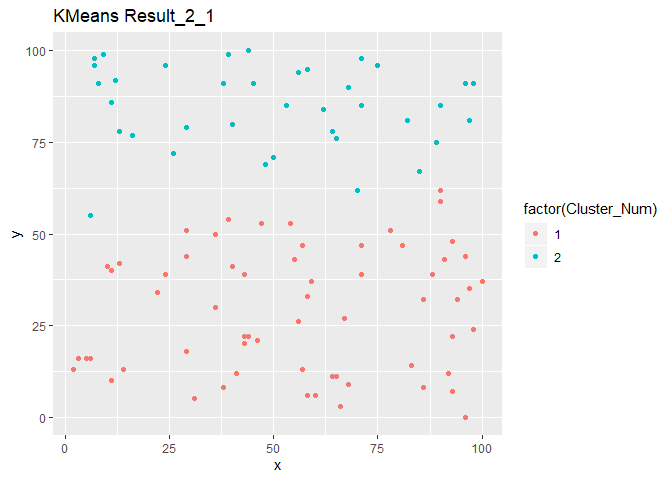
\includegraphics{KMeans_Pic_files/figure-latex/unnamed-chunk-2-1.pdf}
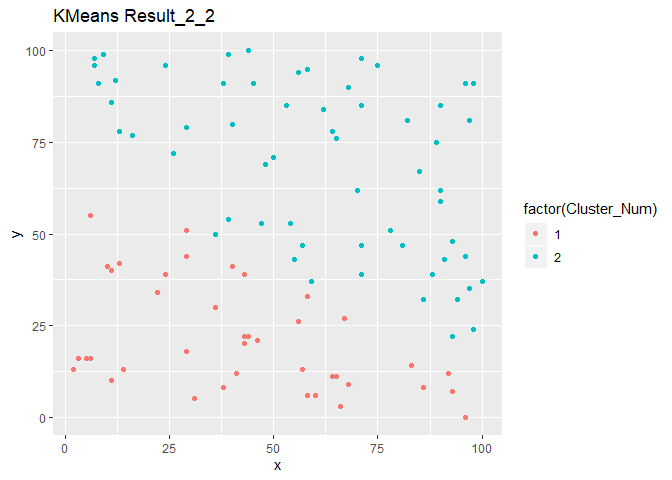
\includegraphics{KMeans_Pic_files/figure-latex/unnamed-chunk-2-2.pdf}
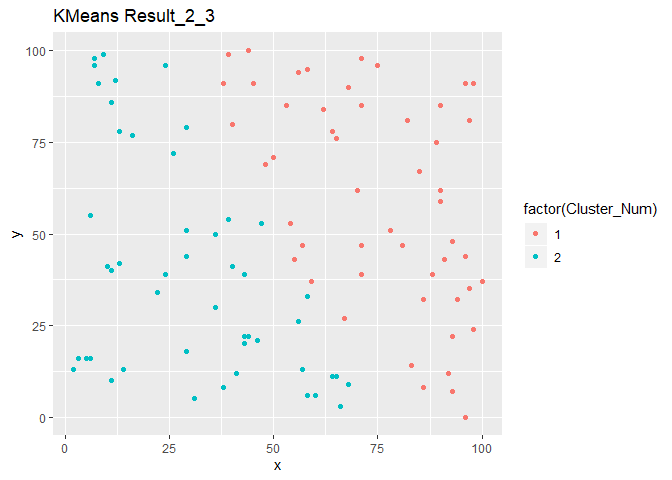
\includegraphics{KMeans_Pic_files/figure-latex/unnamed-chunk-2-3.pdf}
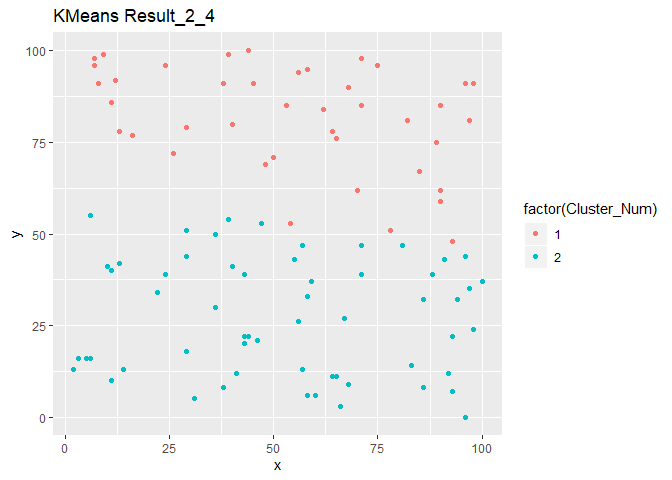
\includegraphics{KMeans_Pic_files/figure-latex/unnamed-chunk-2-4.pdf}
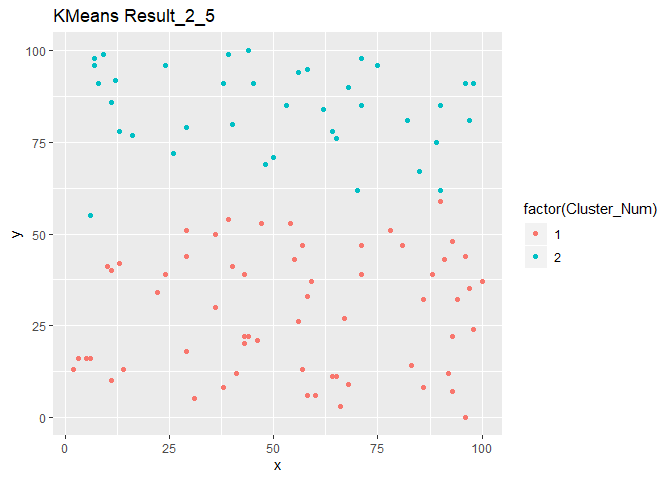
\includegraphics{KMeans_Pic_files/figure-latex/unnamed-chunk-2-5.pdf}
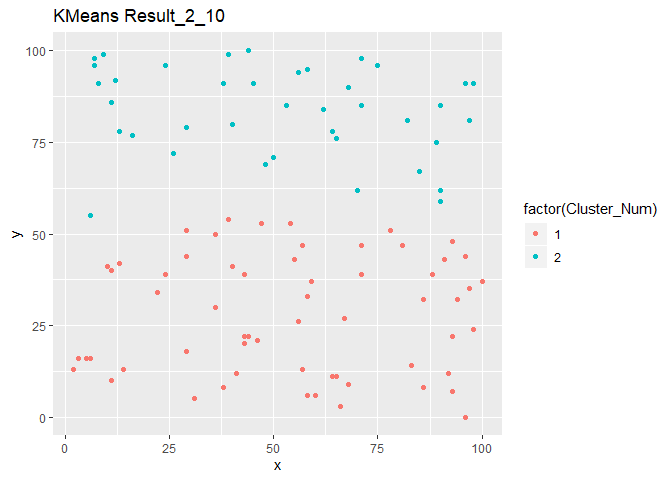
\includegraphics{KMeans_Pic_files/figure-latex/unnamed-chunk-2-6.pdf}
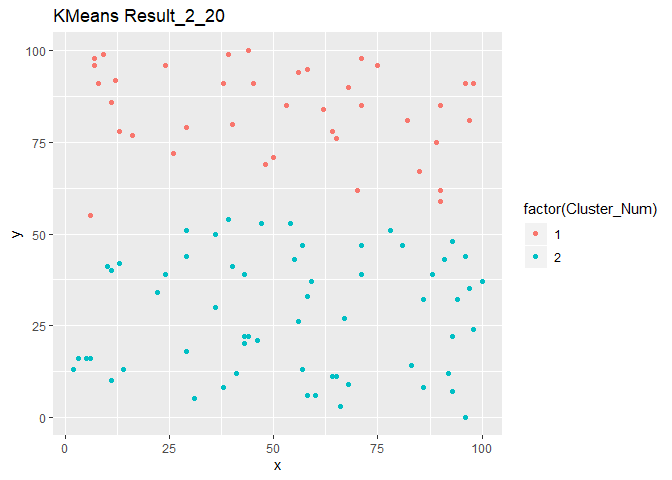
\includegraphics{KMeans_Pic_files/figure-latex/unnamed-chunk-2-7.pdf}
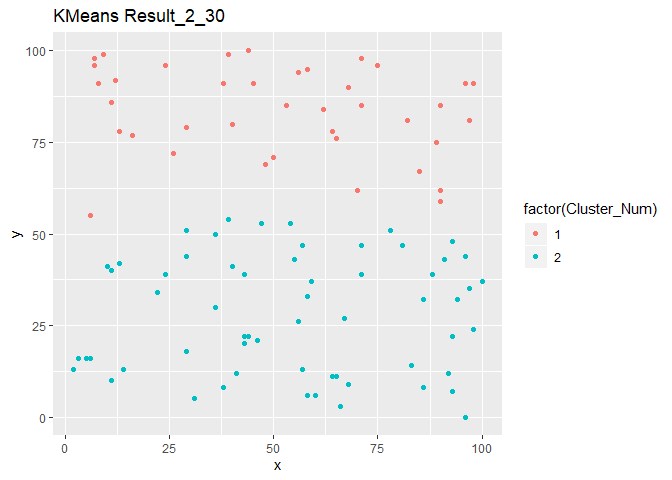
\includegraphics{KMeans_Pic_files/figure-latex/unnamed-chunk-2-8.pdf}
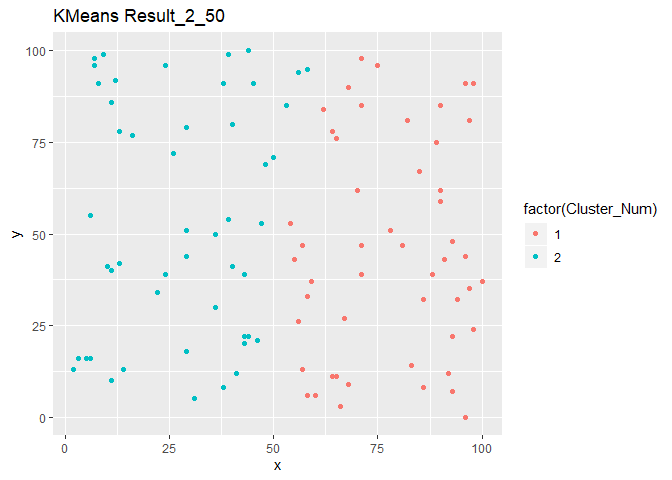
\includegraphics{KMeans_Pic_files/figure-latex/unnamed-chunk-2-9.pdf}
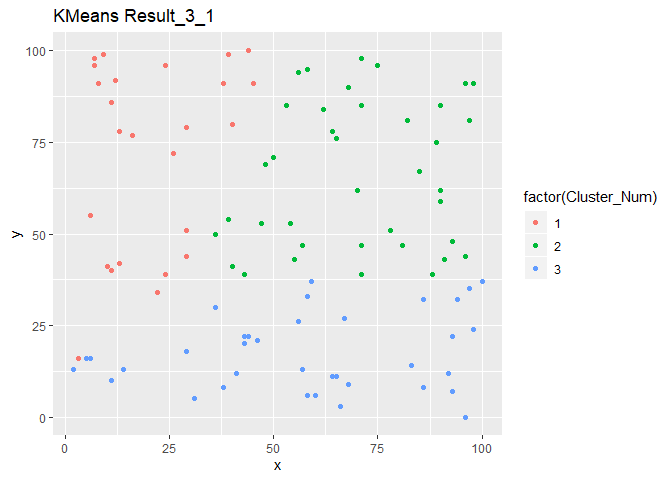
\includegraphics{KMeans_Pic_files/figure-latex/unnamed-chunk-2-10.pdf}
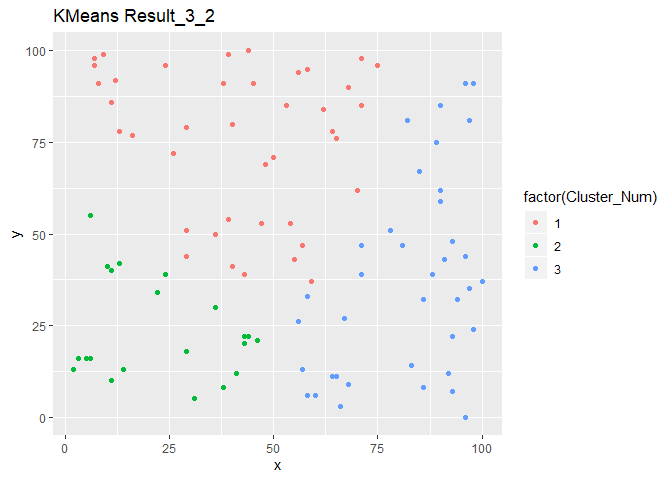
\includegraphics{KMeans_Pic_files/figure-latex/unnamed-chunk-2-11.pdf}
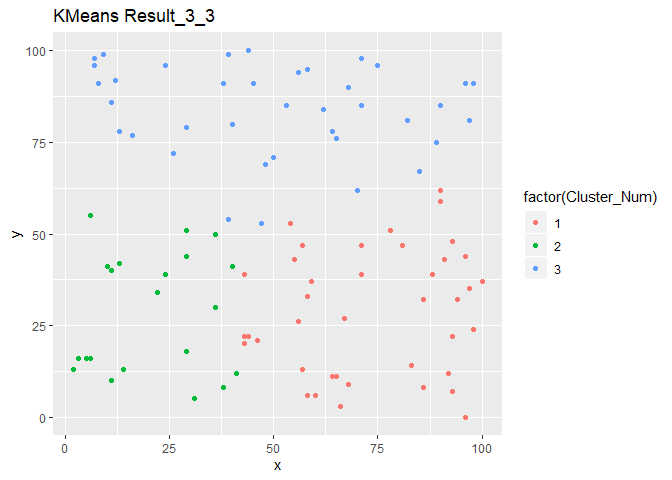
\includegraphics{KMeans_Pic_files/figure-latex/unnamed-chunk-2-12.pdf}
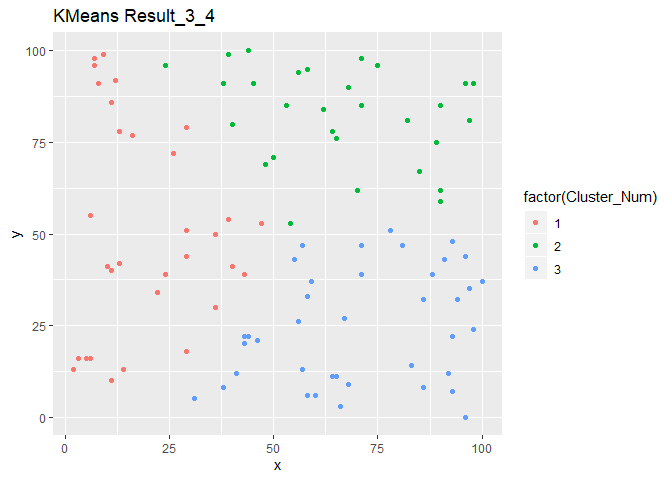
\includegraphics{KMeans_Pic_files/figure-latex/unnamed-chunk-2-13.pdf}
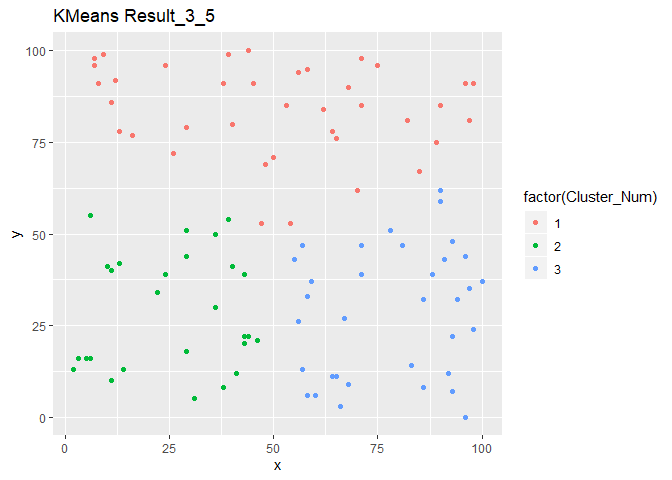
\includegraphics{KMeans_Pic_files/figure-latex/unnamed-chunk-2-14.pdf}
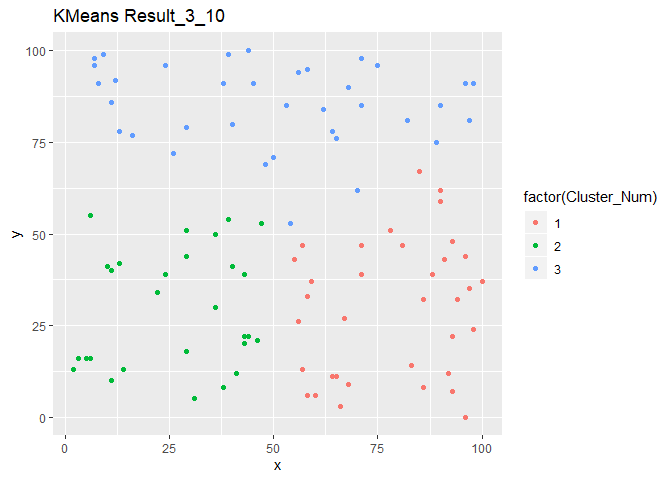
\includegraphics{KMeans_Pic_files/figure-latex/unnamed-chunk-2-15.pdf}
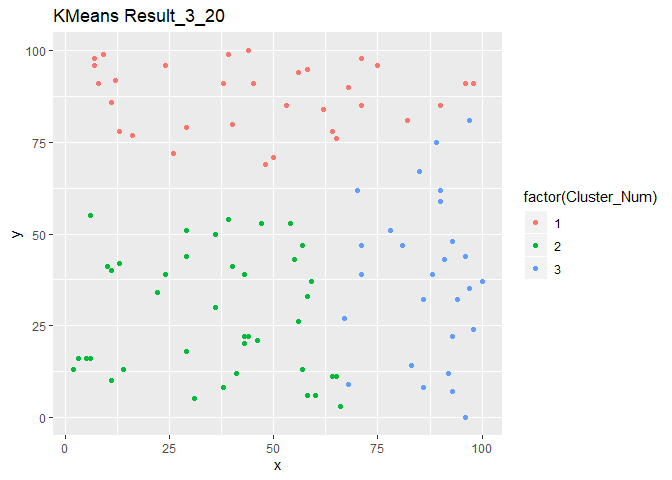
\includegraphics{KMeans_Pic_files/figure-latex/unnamed-chunk-2-16.pdf}
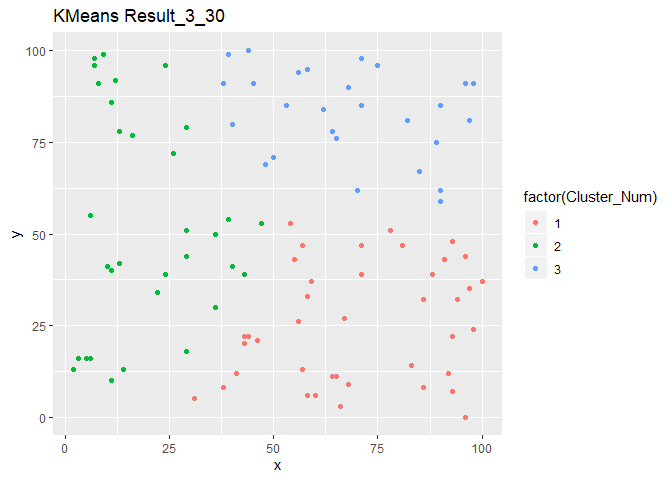
\includegraphics{KMeans_Pic_files/figure-latex/unnamed-chunk-2-17.pdf}
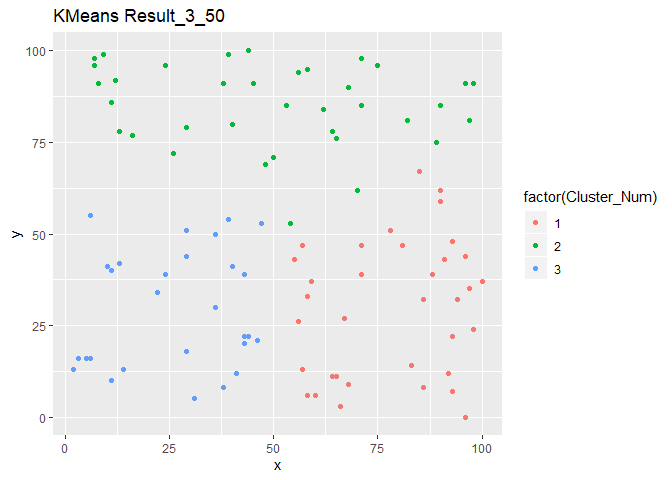
\includegraphics{KMeans_Pic_files/figure-latex/unnamed-chunk-2-18.pdf}
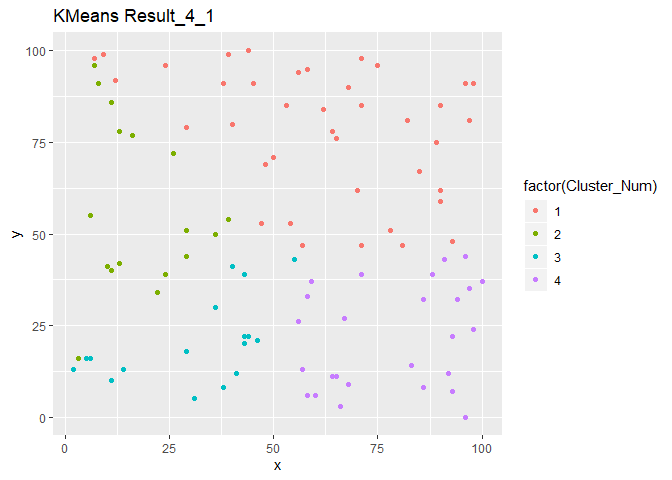
\includegraphics{KMeans_Pic_files/figure-latex/unnamed-chunk-2-19.pdf}
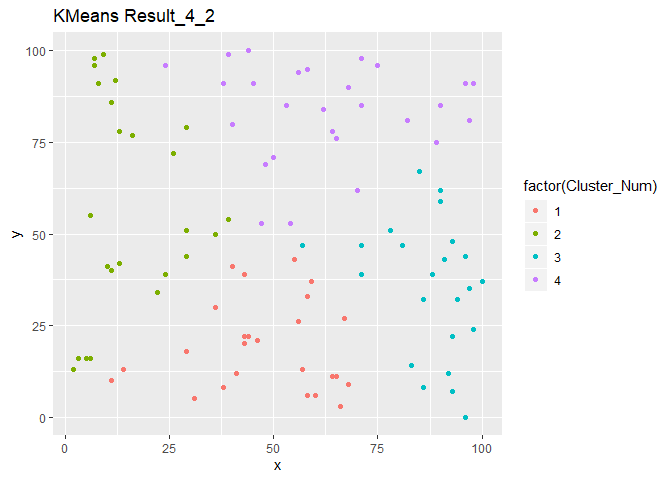
\includegraphics{KMeans_Pic_files/figure-latex/unnamed-chunk-2-20.pdf}
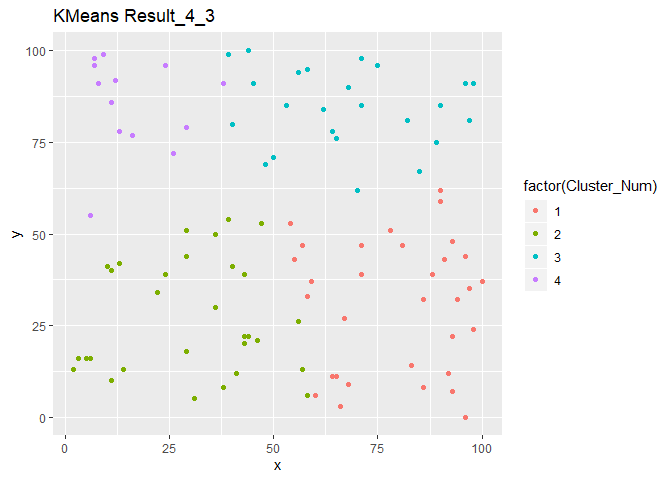
\includegraphics{KMeans_Pic_files/figure-latex/unnamed-chunk-2-21.pdf}
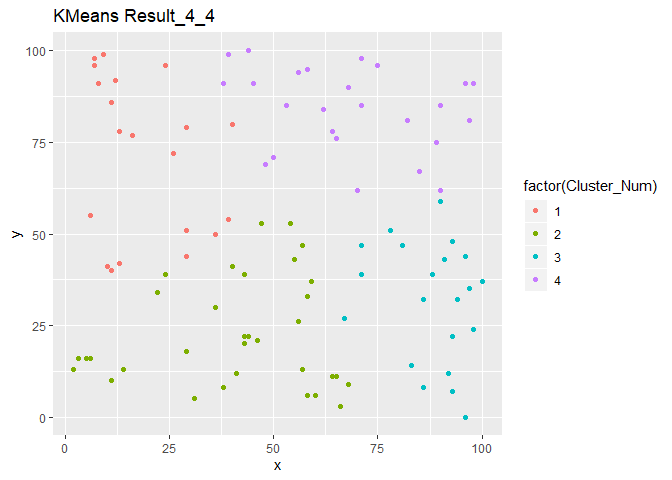
\includegraphics{KMeans_Pic_files/figure-latex/unnamed-chunk-2-22.pdf}
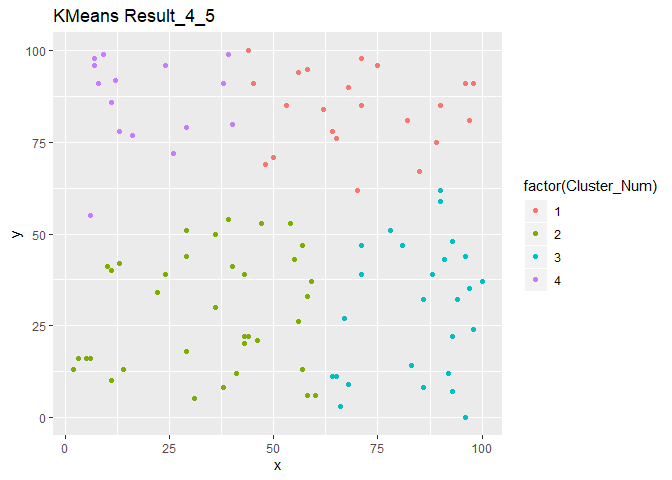
\includegraphics{KMeans_Pic_files/figure-latex/unnamed-chunk-2-23.pdf}
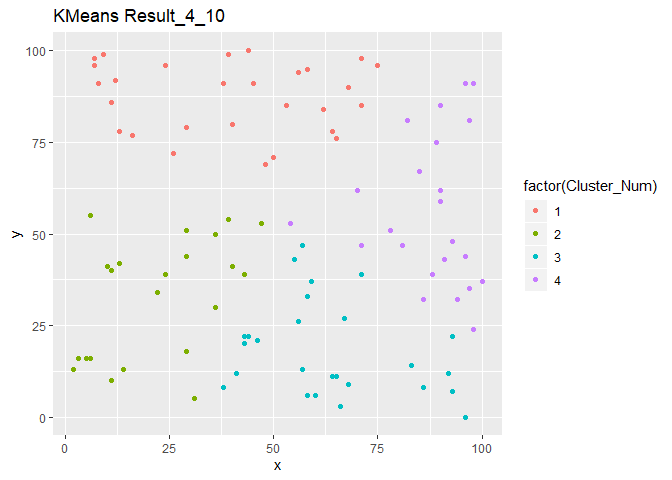
\includegraphics{KMeans_Pic_files/figure-latex/unnamed-chunk-2-24.pdf}
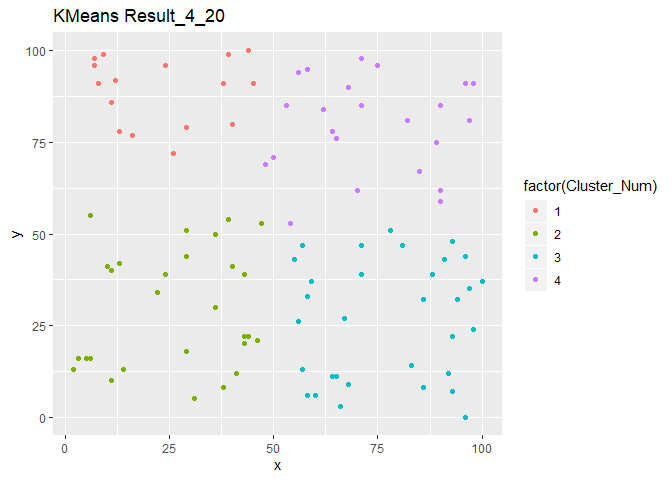
\includegraphics{KMeans_Pic_files/figure-latex/unnamed-chunk-2-25.pdf}
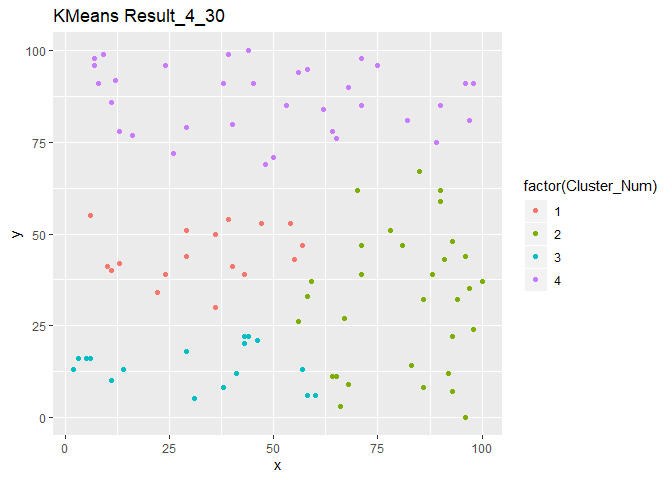
\includegraphics{KMeans_Pic_files/figure-latex/unnamed-chunk-2-26.pdf}
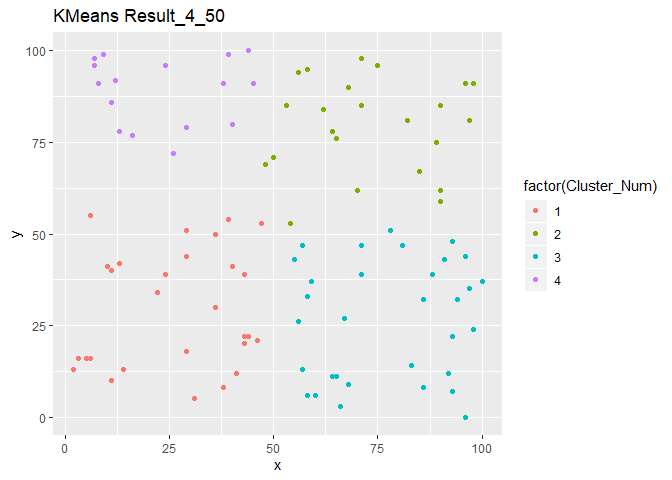
\includegraphics{KMeans_Pic_files/figure-latex/unnamed-chunk-2-27.pdf}
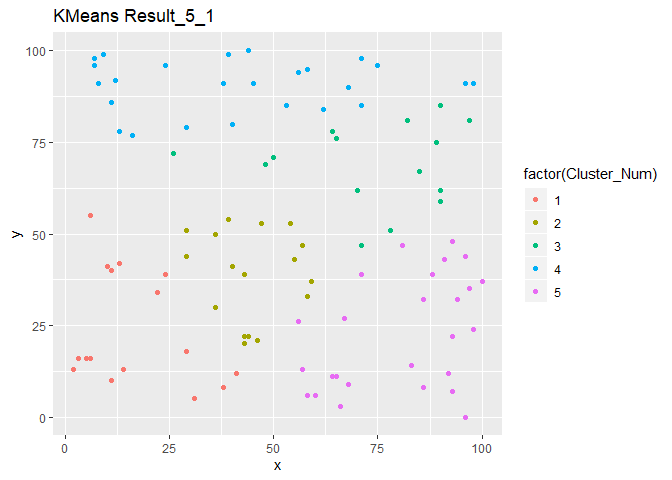
\includegraphics{KMeans_Pic_files/figure-latex/unnamed-chunk-2-28.pdf}
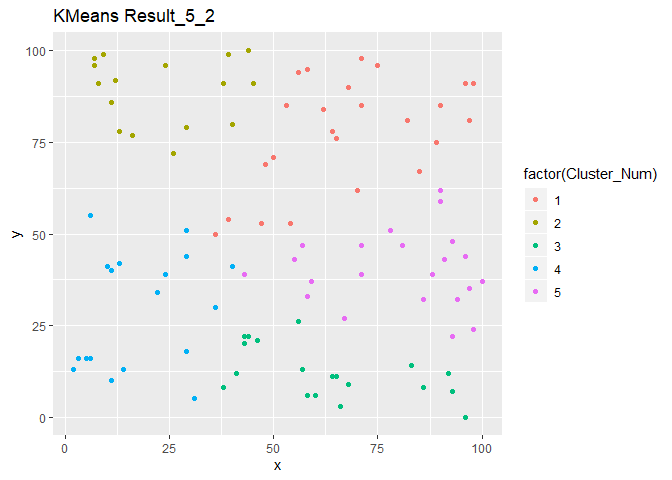
\includegraphics{KMeans_Pic_files/figure-latex/unnamed-chunk-2-29.pdf}
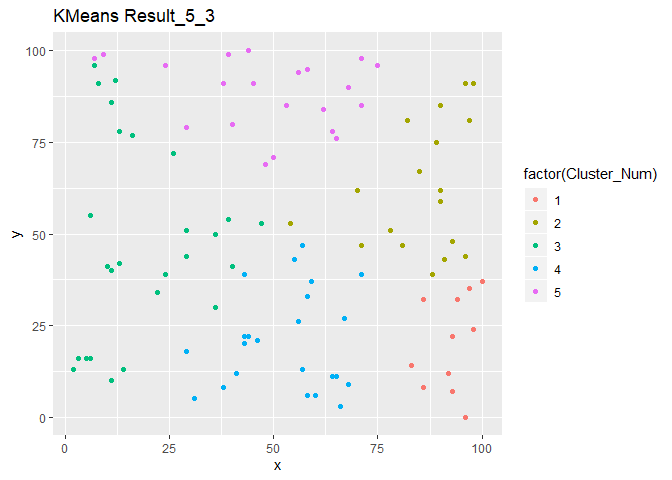
\includegraphics{KMeans_Pic_files/figure-latex/unnamed-chunk-2-30.pdf}
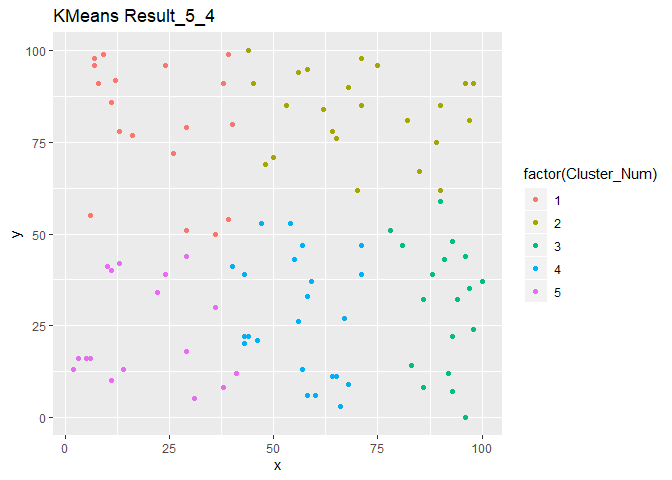
\includegraphics{KMeans_Pic_files/figure-latex/unnamed-chunk-2-31.pdf}
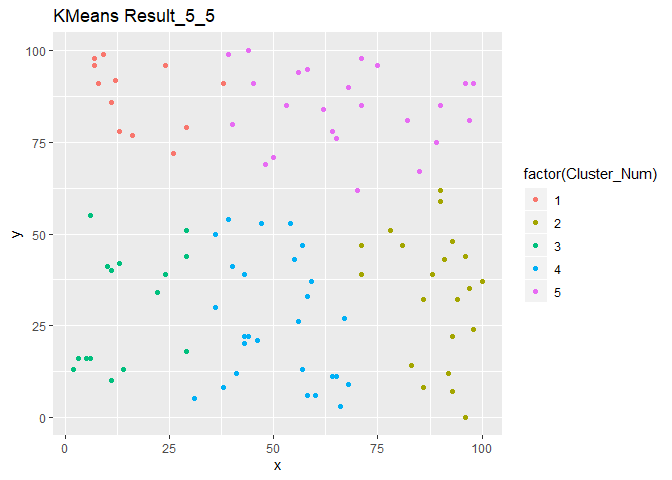
\includegraphics{KMeans_Pic_files/figure-latex/unnamed-chunk-2-32.pdf}
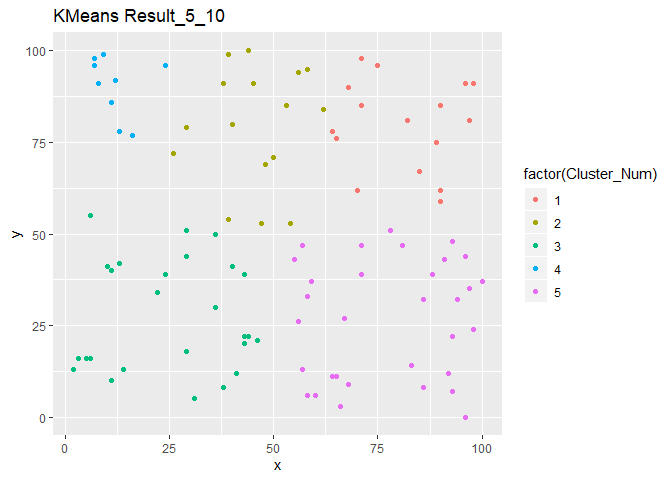
\includegraphics{KMeans_Pic_files/figure-latex/unnamed-chunk-2-33.pdf}
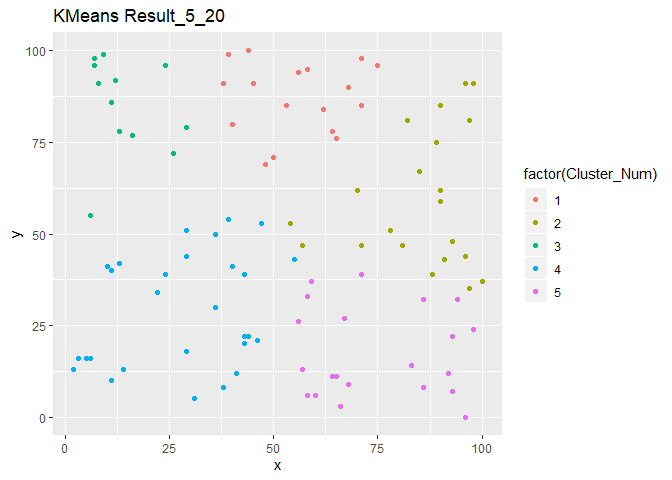
\includegraphics{KMeans_Pic_files/figure-latex/unnamed-chunk-2-34.pdf}
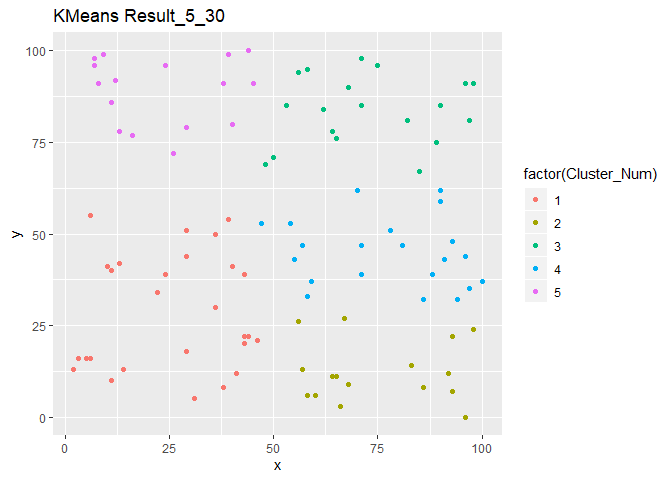
\includegraphics{KMeans_Pic_files/figure-latex/unnamed-chunk-2-35.pdf}
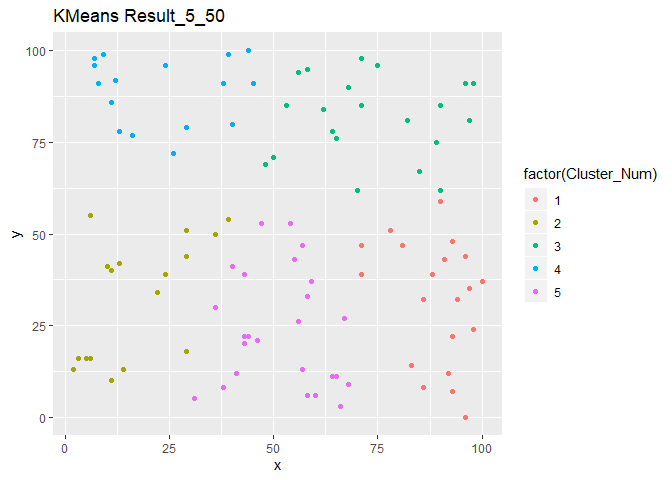
\includegraphics{KMeans_Pic_files/figure-latex/unnamed-chunk-2-36.pdf}


\end{document}
